\chapter{Reinforcement learning} \label{chap:RL}

This chapter shortly explains the working and principles of reinforcement learning (RL)\nomenclature{RL}{Reinforcement Learning} and Deep reinforcement learning (DRL)\nomenclature{DRL}{Deep Reinforcement Learning}.

RL is an area of machine learning (ML) \nomenclature{ML}{Machine Learning} which is a part of artificial intelligence (AI) \nomenclature{AI}{Artificial Intelligence}. In DRL (section \ref{sec:DRL}), RL is mixed with Deep Learning (DL)\nomenclature{DL}{Deep Learning}. This allows to solve much more complex problems.

\section{Markov Decision Processes} \label{sec:MDP}

In RL, an agent performs in and interacts with an environment. This environment is called an Markov decision process (MDP)\footnote{In this paper, the terms "MDP" and "environment" are used interchangeably.} \nomenclature{MDP}{Markov Decision Process}. At every time step, the agent gets an observation of the environment which is a part of the environment's current state or all of it. The agent then chooses an action among a set of actions authorized by the environment and submits it to the environment. This action is chosen according to what is called the agent's policy. Finally, the environment reacts to this action by updating its state and providing the agent with a reward, depending on the previous state and the action performed by the agent. This process then repeats itself until the environment ends up in an end state. An illustration of the agent-environment interactions in an MDP is show on figure \ref{fig:MDP}.\\

\begin{figure}[h!]
    \centering
    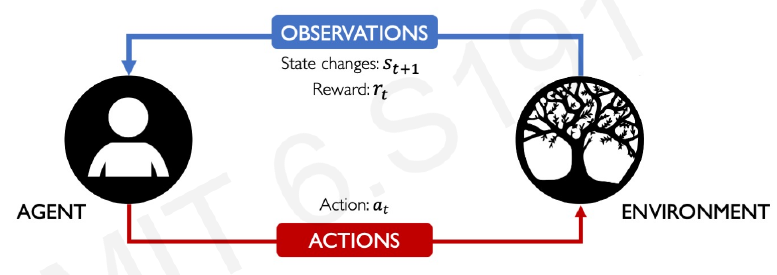
\includegraphics[width=0.7\textwidth]{images/MDP.png}
    \caption{Agent-environment interaction in an MDP \cite{MIT:DL}}
    \label{fig:MDP}
\end{figure}

An MDP is defined by:
\begin{itemize}
    \item A set of states
    \item A set of actions
    \item A transition function
    \item A reward function
    \item A start state
    \item Often one or several terminal state(s)
\end{itemize}


\subsection{Transition function} \label{sec:transition function}

The transition function $T(s,a,s')$ is the probability that taking action $a$ in state $s$ will lead to stats $s'$, i.e.:\nomenclature{$T(s,a,s')$}{Transition function of an MDP}

\begin{equation} \label{eq:transition function}
    T(s,a,s') = P(S_{t+1}=s'|S_t=s,A_t=a) 
\end{equation}

\subsection{Reward function} \label{sec:reward function}

The reward function $R(s,a,s')$ is the reward you get by that taking action $a$ in state $s$ and end up in state $s'$.\nomenclature{$R(s,a,s')$}{Reward function of an MDP}\\

In some MDPs, the reward only depends on the state he agent ends up in and is thus noted $R(s)$.

\section{Concepts and definitions}

\subsection{Discounted factor and discounted cumulative reward}\label{sec:gamma}

Very often, a discount factor $\gamma\ (0\leq \gamma \leq 1$) \nomenclature{$\gamma$}{Discount Factor} is introduced. We then talk about the cumulative discounted reward $G_t$\nomenclature{$G_t$}{Cumulative Discounted Reward}, which is expressed as follows:

\begin{align} \label{eq:discounted reward}
    G_t &= \sum _{k=0}^\infty \gamma ^k R_ {t+k+1}\\
        &= R_{t+1} + \gamma G_{t+1}
\end{align}

The agent must then choose the actions that optimize $G_t$. introducing this $\gamma$ models the uncertainty of the future rewards and helps our algorithm to converge. 

\subsection{Policy}

The policy $\pi(s)$ \nomenclature{$\pi$}{Policy} is a function that returns an action a to take in state s. In a more general way, it can also give a probability distribution over all available actions in state s. If that is the case, it will be denoted $\pi(a|s)$. The optimal policy, i.e. the one that optimized (\ref{eq:discounted reward}) is $\pi^*(s)$ \nomenclature{$\pi^*$}{Optimal Policy}.

\subsection{Value and Q-value}\label{sec:value}

The value of a state $V_\pi(s)$ \nomenclature{$v_\pi(s)$}{Value of state s under policy $\pi$} is the expected (discounted) cumulative reward when starting from state s and choosing action with policy $\pi$. 
\begin{equation} \label{eq:value}
    V_\pi(s) = \mathbb{E}_{\pi}[G_t|S_t=s]
\end{equation}
$V_{\pi^*}(s)$ or $V_*(s)$ is the value of state s under the optimal policy.\\ \nomenclature{$V_*(s)$}{Value of state s under optimal policy}


The Q-value of a state-action pair $Q_\pi(s,a)$ \nomenclature{$Q_\pi(s,a)$}{Q-value of state-action pair (s,a) under policy $\pi$} is the expected (discounted) cumulative reward when starting from state a and undertaking action a, then acting according to policy $\pi$.
\begin{equation} \label{eq:q-value}
    Q_\pi(s,a) = \mathbb{E}_{\pi}[G_t|S_t=s,A_t=a]
\end{equation}
As for the state value, $Q_{\pi^*}(s,a)$ or $Q_*(s,a)$ is the Q-value of state-action pair (s,a) under the optimal policy. Sometimes, a state-action pair is also called a q-state.\\ \nomenclature{$Q_*(s,a)$}{Q-value of state-action pair (s,a) under optimal policy}

The link between value and q-value is then:
\begin{equation}
    V_\pi(s) = Q_\pi(s,\pi(s))
\end{equation}

Or, with the optimal policy:
\begin{equation}
    V_*(s) = \max_a Q_*(s,a)
\end{equation}

\subsection{Episode and transition} \label{sec:episodes and transitions}

An episode in an MDP is one specific sequence of states actions and reward that starts with the start state of the environment end stops with a terminal state. 

In a MDP, moving from one state to another is called a transition. More specifically when we talk about a transition in RL, it can be (and will be for the rest of this thesis) a sample of one time step of a particular episode. The transition at time t contains the following data:\\

\begin{itemize}
    \item $S_t$ the state (or local observation) at time step t.
    \item $A_t$ the action performed by the agent at time step t.
    \item $R_t$ the reward received by the agent at time step t.
    \item $S_{t+1}$ the state (or local observation) at time step t+1.
    \item $is\_done$ a Boolean value that is true only if $S_t$ is terminal. $S_{t+1}$ will then be None or 0.
\end{itemize}

\subsection{Bellman equation}

It can be shown that the Q-value function of the optimal policy $Q_*(s,a)$ obeys a recursive relationship that is called the Bellman equation:

\begin{align}\label{eq:bellman}
    Q_*(s,a) &= \sum_{s'} T(s,a,s') [R(s,a,s')+\gamma \max_{a'}Q(s',a')]\\
             &= \sum_{s'} T(s,a,s') [R(s,a,s')+\gamma V(s')]
\end{align}

The optimal policy can than easily be retrieved from $Q_*(s,a)$:
\begin{equation} \label{eq:pi from Q}
    \pi_*(s) = \argmax_a Q_*(s,a)
\end{equation}


\section{Tabular Q-learning}

So, in RL, we want to find that optimal policy, that is, the one that maximizes (\ref{eq:discounted reward}). One easy algorithm to do so is called Q-learning. As the name suggests, the algorithm will try to learn the Q-values for every state and action for the MDP in which it is learning. The optimal policy will then be retrieved with (\ref{eq:pi from Q}).\\

\subsection{The Algorithm} \label{sec:Q-learning}

First, a table is created. This table contains the estimations of the Q-values for every possible state and action in the environment. It can be initiated with random values or zeros. This table is called the Q-table. An example of such a table for an environment with N states and M actions is show on figure \ref{fig:Q-table}.\\

\begin{figure}
    \centering
    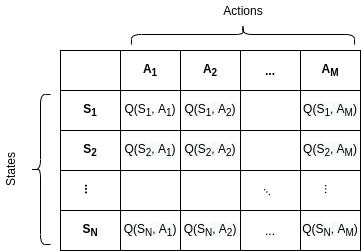
\includegraphics[width=.55\textwidth]{images/Q-table.png}
    \caption{Example of a Q-table in Q-learning \cite{Q-learning}}
    \label{fig:Q-table}
\end{figure}

Then, the agent will perform in the environment, collecting data in the form of transitions. For each transition, the agent "learns" by updating its Q-table using (\ref{eq:q-learning}), inspired by (\ref{eq:bellman}).

\begin{equation} \label{eq:q-learning}
    Q(S_t,A_t) \leftarrow Q(S_t,A_t) + \alpha [R_t + \gamma \max_a Q(S_{t+1},a) - Q(S_t,A_t)] 
\end{equation}

where:
\begin{itemize}
    \item $\alpha\ (0 < \alpha < 1)$ \nomenclature{\alpha}{Learning rate} is the learning rate.
    \item $[R_t + \gamma \max_a Q(S_{t+1},a) - Q(S_t,A_t)]$ is the temporal difference. It is actually the difference between what $Q(S_t,A_t)$ should be (i.e. $R_t + \gamma \max_a Q(S_{t+1},a)$) and what it really is. 
\end{itemize}\hfill\break
At every learning step, that is, at every transition, $Q(S_t,A_t)$ is incremented by the temporal difference multiplied by the learning rate. If $\alpha = 1$, the agent ignores prior knowledge and $Q(S_t,A_t)$ is replaced by the temporal difference at every learning step. If $\alpha = 0$, the agent is not learning at all. The learning rate actually determines how fast the Q-values in the Q-table will change. A higher learning rate might lead to faster convergence of our Q-values towards the optimal values, but a too high learning rate might also lead to no convergence at all.\\

If $S_t$ is a terminal state, \ref{eq:q-learning} becomes: 

\begin{equation}
    Q(S_t,A_t) \leftarrow Q(S_t,A_t) + \alpha [R_t - Q(S_t,A_t)] 
\end{equation}


\subsection{The epsilon-greedy policy} \label{sec:eps-greedy}

As explained in previous section, the agent learns by performing in its environment. While it does this, it updates its q-table with the data obtain from the environment at every transition. Thus, the different states visited by the agent have a really important impact on the quality of the learning. Those visited states depend on the actions the agent decides to perform, which are determined by its policy. Hence, besides the learning process, the agent's policy is also really important in the learning process.\\

It might seem a good option to use (\ref{eq:pi from Q}), but using the agent's Q-table instead of the optimal Q-values function $Q_*(s,a)$, which is unknown. However, following that sub-optimal policy might lead to an agent that explores only certain states. If the environment gives some high reward when going to certain states, but the agent never goes to those states, the Q-values for those states will never be updated to higher values and the agent will never learn the optimal policy.\\

Thus, the agent shall explore every state during the learning. A solution to that is the epsilon-greedy policy. At every transition, the probability that the agent will choose an action using (\ref{eq:pi from Q}) with its own Q-table is $1-\epsilon$. And there is an $\epsilon$ probability that the agent will take a random action from all available actions in the environment. It is obvious that $\epsilon$ is a really important parameter in the epsilon-greedy policy and that $0 \leq \epsilon \leq 1$.

\subsection{The exploration/exploitation dilemma}

The exploration/exploitation dilemma is a problem that is often encountered in RL. As already stated in section \ref{sec:eps-greedy}, we have to add some randomness in the chosen actions in order to allow the agent to explore all of the possible states. That is what is called exploration.\\

However, in some more complex environment, there are states in which the agent is very unlikely to find itself by performing only random actions. Let's take the example of a video game where you have several levels: if you play randomly, you could get some little rewards if you start to progress in the correct direction. But, if the game is complex, it is very unlikely that the agent will finish the whole level and access the next ones by playing randomly. Hence, the agent will never observe the more advanced states, further in the game. So, at a certain moment, the agent has to exploit what it has already learnt in order to access some other states and explore the results of action undertaken in those states. This is called the exploitation.\\

The dilemma is thus to find a good equilibrium between exploration and exploitation, in order to be sure to explore every possibility, but still advanced to the states that are more difficult to access. One solution to this problem is to implement an epsilon decay. The idea is to decrease the value of the epsilon parameter of the agent's epsilon-greedy policy as the episodes progress. This way, the agent will act more randomly in the start of the training, when it hasn't learnt much, but will act more and more according to its q-table, as the values of that table converge to the optimal solution.